\documentclass[a4paper,11pt]{report}
\usepackage[slovene]{babel}
\usepackage{listings}
\usepackage{graphicx}
\usepackage[section]{placeins}
\usepackage{footnote}
\makesavenoteenv{tabular}

\newcommand{\ttitle}{Vzorec bla dela}
\newcommand{\tauthor}{Matjaž Kralj}
\newcommand{\autfont}{\Large}
\newcommand{\titfont}{\LARGE\bf}

\lstset{
numberstyle=\small, 
numbersep=8pt, 
frame = single, 
language=SQL, 
framexleftmargin=15pt}

\begin{document}


\thispagestyle{empty}
\begin{center}
    {\large\sc Univerza v Ljubljani\\%
      Fakulteta za računalništvo in informatiko}%
    \vskip 10em%
    {\autfont Jakob Marušič\par}%
    {\titfont Primerjava performance SQL podatkovnih baz \par}%
    {\vskip 3em Seminarska naloga pri predmetu Tehnologija upravljanja podatkov\\\par}%
    \vfill\null%
    %{\large \textsc{Mentor}: doc.\ dr.  Peter Klepec\par}%
    {\vskip 2em \large Ljubljana, 2020 \par}%
\end{center}

\chapter*{Uvod}

V poplavi različnih sistemov za upravljanje s podatkovnimi bazami (SUPB) razvijalci pogosto izbirajo 
glede na dosedanje izkušnje pri delu s SUPB-ji ali glede na poslovna pravila določena s strani organizacije.
\paragraph{}
Odločitev je pogosto sprejeta s predpostavko, da večina rešitev za upravljanje s podatki omogoča primerjivo performanco.
V seminarski nalogi, ki je nastala v okviru predmeta Tehnologija upravljanja podatkov, želim preveriti to predpostavko s testiranje primerjivih operacij v različnih SUPB-jih.

\paragraph{}
Vsi testi v nadaljevanju te seminarske naloge temeljijo na predpostavki, da razvijalca nekega sistema ne zanima optimizacija na ravni podatkovne baze.
Zaradi tega se nastavitev testiranih baz pred začetkom testa ni spreminjalo, uporabljalo pa se je zgolj osnovno SQL sintakso (in ne posebnih SQL ukazov, ki so prisotni
pri nekaterih SUPB-jih in lahko omogočajo bolj optimizirane operacije, primer \textit{BULK INSERT} pri MSSQL Server). 
Ravno tako so testi narejeni na predpostavki, da ima SUPB na voljo dovolj zmogljivo strojno arhitekturo in ni omejen z delovnim pomnilnikom ali CPU.
\pagebreak

\chapter{Način testiranja}
\section{Izbrani SUPB}
Testiranje se bo izvajalo na štirih prosto dostopnih podatkovnih bazah: MySQL, MariaDB, PostgreSQL in Micorsoft SQL Server Express \textit{(v nadaljevanju Microsoft SQL Server, MSSQL Server)}.
\\\\
Vse štiri podatkovne baze se bodo izvajale istočasno na Dockerju.

\subsection{Zagon Docker slik}

\subsection{MySql}
\begin{lstlisting}
docker run --name TUP-sem-mysql -p 7202:3306 -e 
        MYSQL_ROOT_PASSWORD=root -d mysql:latest
\end{lstlisting}

Baza je dostopna na naslovu http://localhost:7202

\subsection{MariaDB}
\begin{lstlisting}
   docker run --name TUP-sem-mariadb -p 7203:3306 -e 
           MYSQL_ROOT_PASSWORD=root -d mariadb:latest
   \end{lstlisting}
   
   Baza je dostopna na naslovu http://localhost:7203

\subsection{PostgreSQL}
\begin{lstlisting}
docker run --name tup-sem-postgres 
      -e POSTGRES_USER=root -e POSTGRES_PASSWORD=root 
      -p 7200:5432 -d postgres
\end{lstlisting}
   
Baza je dostopna na naslovu http://localhost:7200

\subsection{Microsoft SQL Server Express}
\begin{lstlisting}
docker run -e 'ACCEPT_EULA=Y' --name tup-sem-mssql 
   -e 'SA_PASSWORD=root_ROOT' -p 7201:1433 
   -d mcr.microsoft.com/mssql/server:2017-CU8-ubuntu
\end{lstlisting}
   
Baza je dostopna na naslovu http://localhost:7201.

\section{Način poganjanja podatkovne baze}
Podatkovna baza je bila nameščena in se je izvajala na računalniku s sledečimi specifikacijami:

\begin{center}
    \begin{tabular}{||l|l||}
        \hline
        Procesor & Intel Core i7-8705G 3.10GHz\\
        \hline
        Delovni pomnilnik (od tega Docker) & 16 GB (6,31GB)\\
        \hline
        Virtualni delovni pomnilnik & 28,9 GB\\
        \hline
        Operacijski sistem & Windows 10 Education\\
        \hline
        Verzija operacijskega sistema & 10.0.18363 Build 18363\\
        \hline
        Verzija Docker okolja\footnote{https://docs.docker.com/docker-for-windows/install/} & 19.03.5\\
        \hline
        Verzija MySQL docker slike \footnote{https://hub.docker.com/\_/mysql} & 8.0.18 \\
        \hline
        Verzija PostgreSQL docker slike\footnote{https://hub.docker.com/\_/postgres} & 12.1\\
        \hline
        Verzija MS SQL Server docker slike\footnote{https://hub.docker.com/\_/microsoft-mssql-server} & 2017\\
        \hline
        Verzija MariaDB docker slike\footnote{https://hub.docker.com/\_/mariadb} & 10.4.11-bionic\\
        \hline
    \end{tabular}
\end{center}
\paragraph{}
\pagebreak

\section{Način točkovanja testiranja in vrste testov}

Vsak test se točkuje z določenim številom točk pri čemer je maksimalno število točk določeno po ključu, kjer je glavni faktor pogostost izvajanja določene operacije v realnem svetu \textit{(primer: zdravstveni dom)}.
\\\\
Testira se vse vidike operacij nad podatki podatkovne baze, katere izvajamo v okviru \textit{CRUD (Create, Read, Update, Delete)} operacij.

\begin{center}
   \begin{tabular}{||c|c|c||}
      \hline
      \textbf{Operacija} & \textbf{Maksimalno število točk} & \textbf{Primer uporabe}\\
      \hline
      \hline
      Vstavljanje\footnote{Vstavljanje velike količine podatkov} podatkov & 25 & migracija podatkov\\
      Brisanje\footnote{Brisanje velike količine podatkov} podatkov & 25 & praznjenje tabel\\
      Posodabljanje\footnote{Posodabljanje velike količine podatkov} podatkov & 50 & spremeba KZZ \\
      Branje, analiza podatkov & \(4 \cdot 50 = 200\) & statistika\\
      \hline
   \end{tabular}
\end{center}

\section{Način izvedbe testov in določitve točk}
Pri vsakem testu, ki se bo izvedel večkrat, bomo po definiranem ključu določili zmagovalca, ki v dani kategoriji dobil maksimalno število točk. Naslednje podatkovne baze pa bodo od maksimalnega števila točk dobila odbitek, ki je enak odstotku razlike med lastnim rezultatom in rezultatom zmagovalca kategorije. 
\\\\
V zaključku raziskave se bodo točke seštele in tako objektivno določile performančnega zmagovalca testov. Vseeno pa so točke podeljene zgolj informativne narave, saj se izkaže, da pri izbiri pravega SUPB-ja ni pomembna zgolj performanca, temveč tudi izbira posameznika, naj si bo naročnika, upravljalca ali programerja podatkovne baze. Več o tem sledi v zaključku naloge. 

\chapter{Podatkovna baza - zdravstveni dom}


\section{Konceptni model}
Podatkovna baza za potrebe testiranja je podatkovna baza zdravstvenega doma, ki se je uporabljala pri 3. domači nalogi.
Podatkovna baza je razdeljena na 7 tabel in ima skupno 1 028 883 vrstic.

\begin{figure}[htb]
    \noindent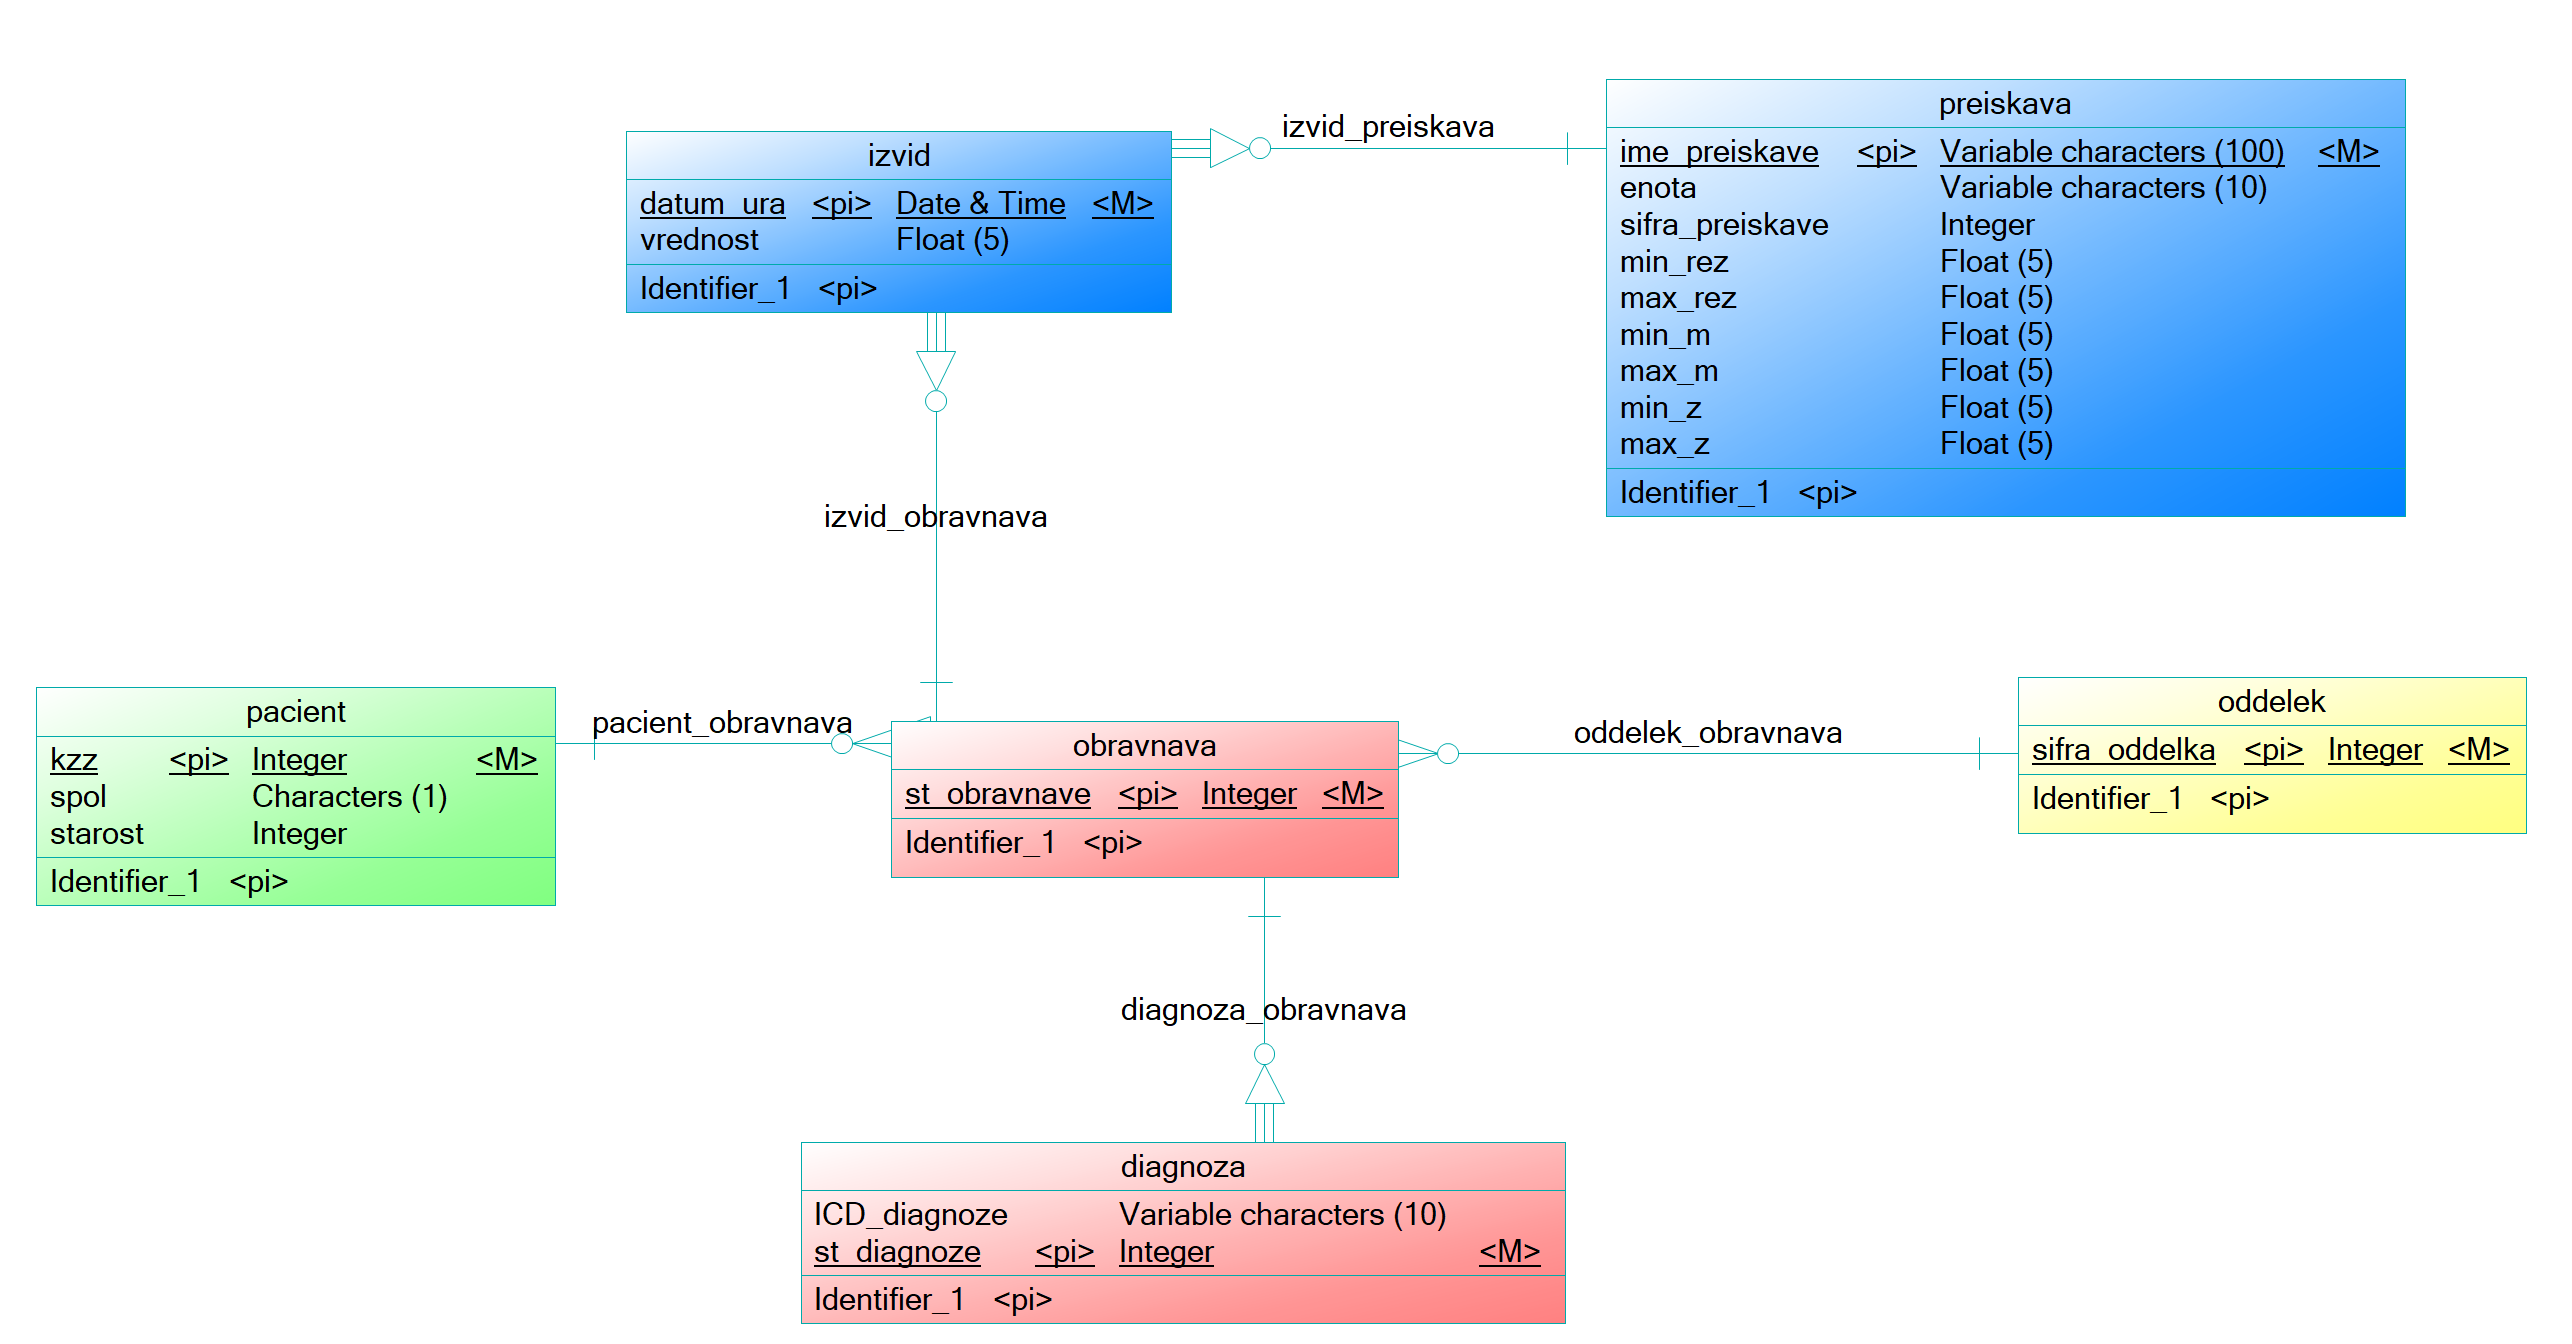
\includegraphics[width=\linewidth]{./pics/konceptni.png}
    \caption{Konceptni model podatkovne baze}
 \end{figure}

\section{Fizični model}
\subsection{MySQL in MariaDB}
\begin{figure}[htb]
   \noindent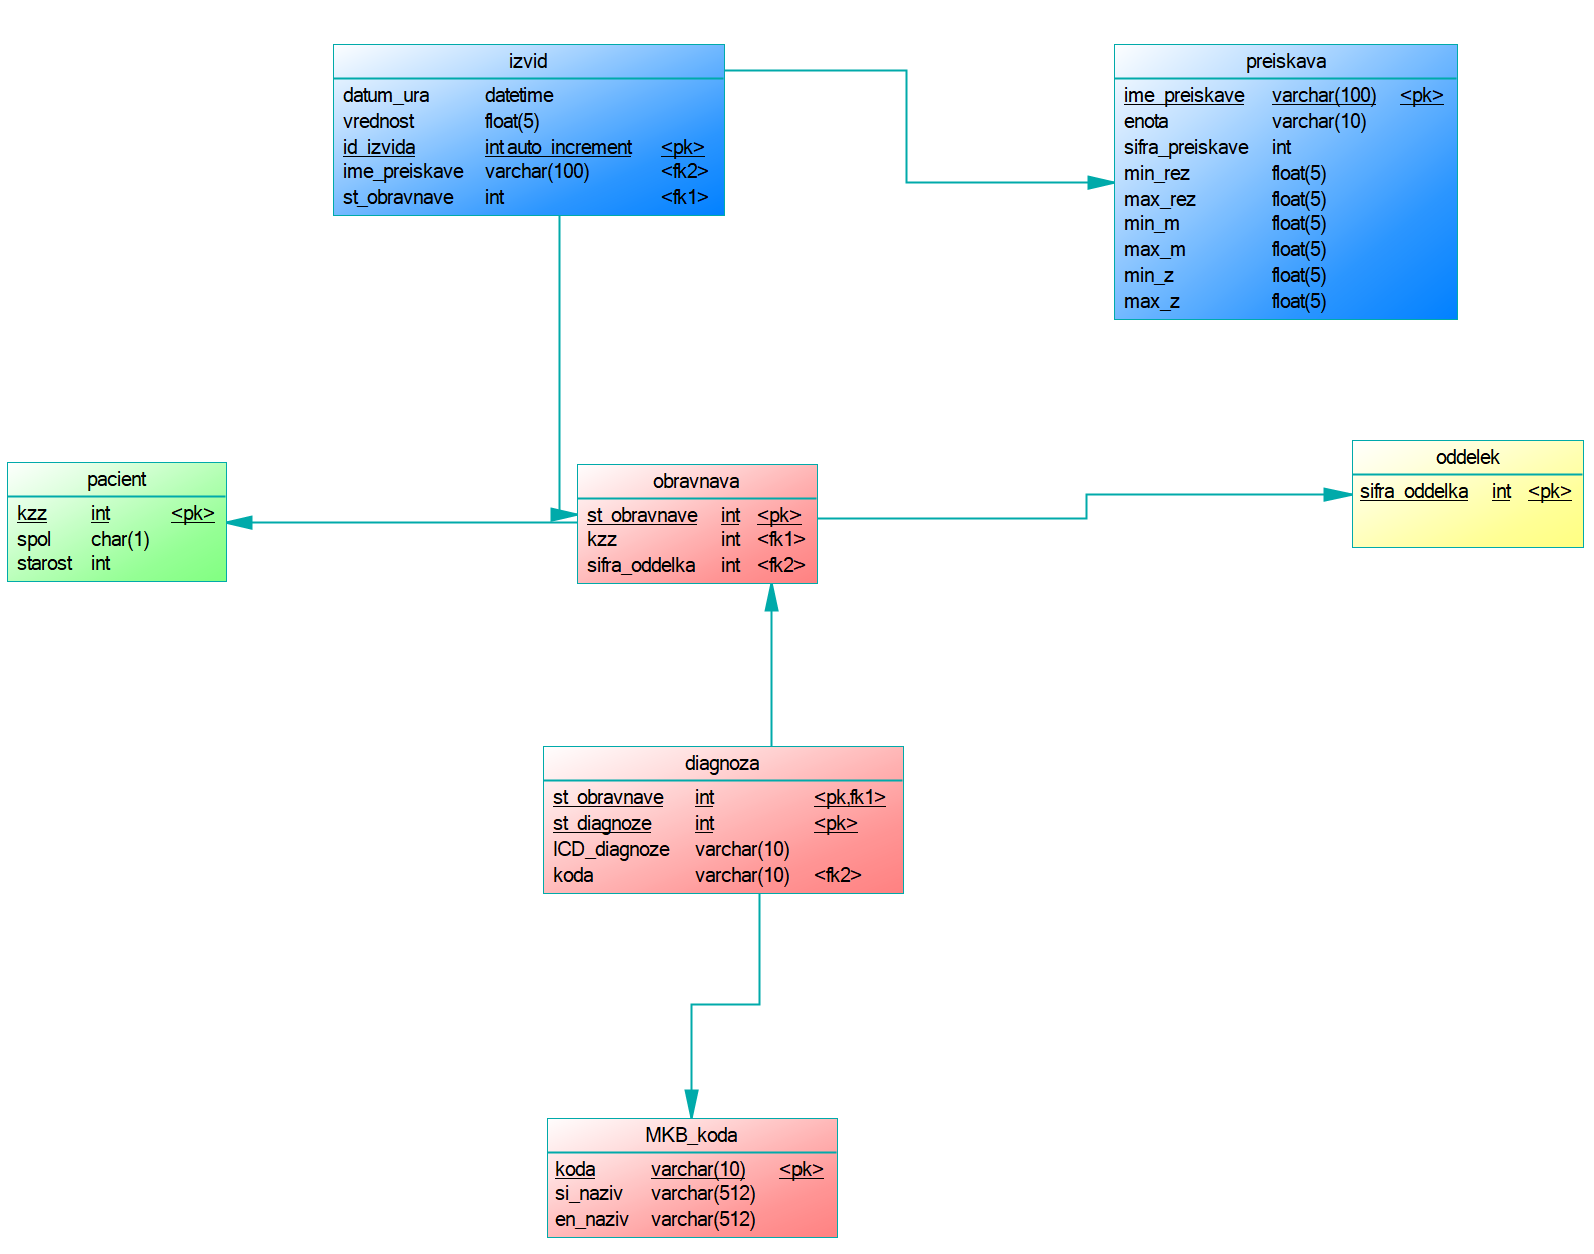
\includegraphics[width=\linewidth]{./pics/fizicni-mysql.png}
   \caption{Fizični model podatkovne baze za MySQL in MariaDB}
\end{figure}
Skripta za ustvarjanje podatkovne baze je shranjena v datoteki \textit{\underline{./sql-skripte/mysql-init.sql}}.
\pagebreak
\subsection{PostgreSQL}
\begin{figure}[htb]
   \noindent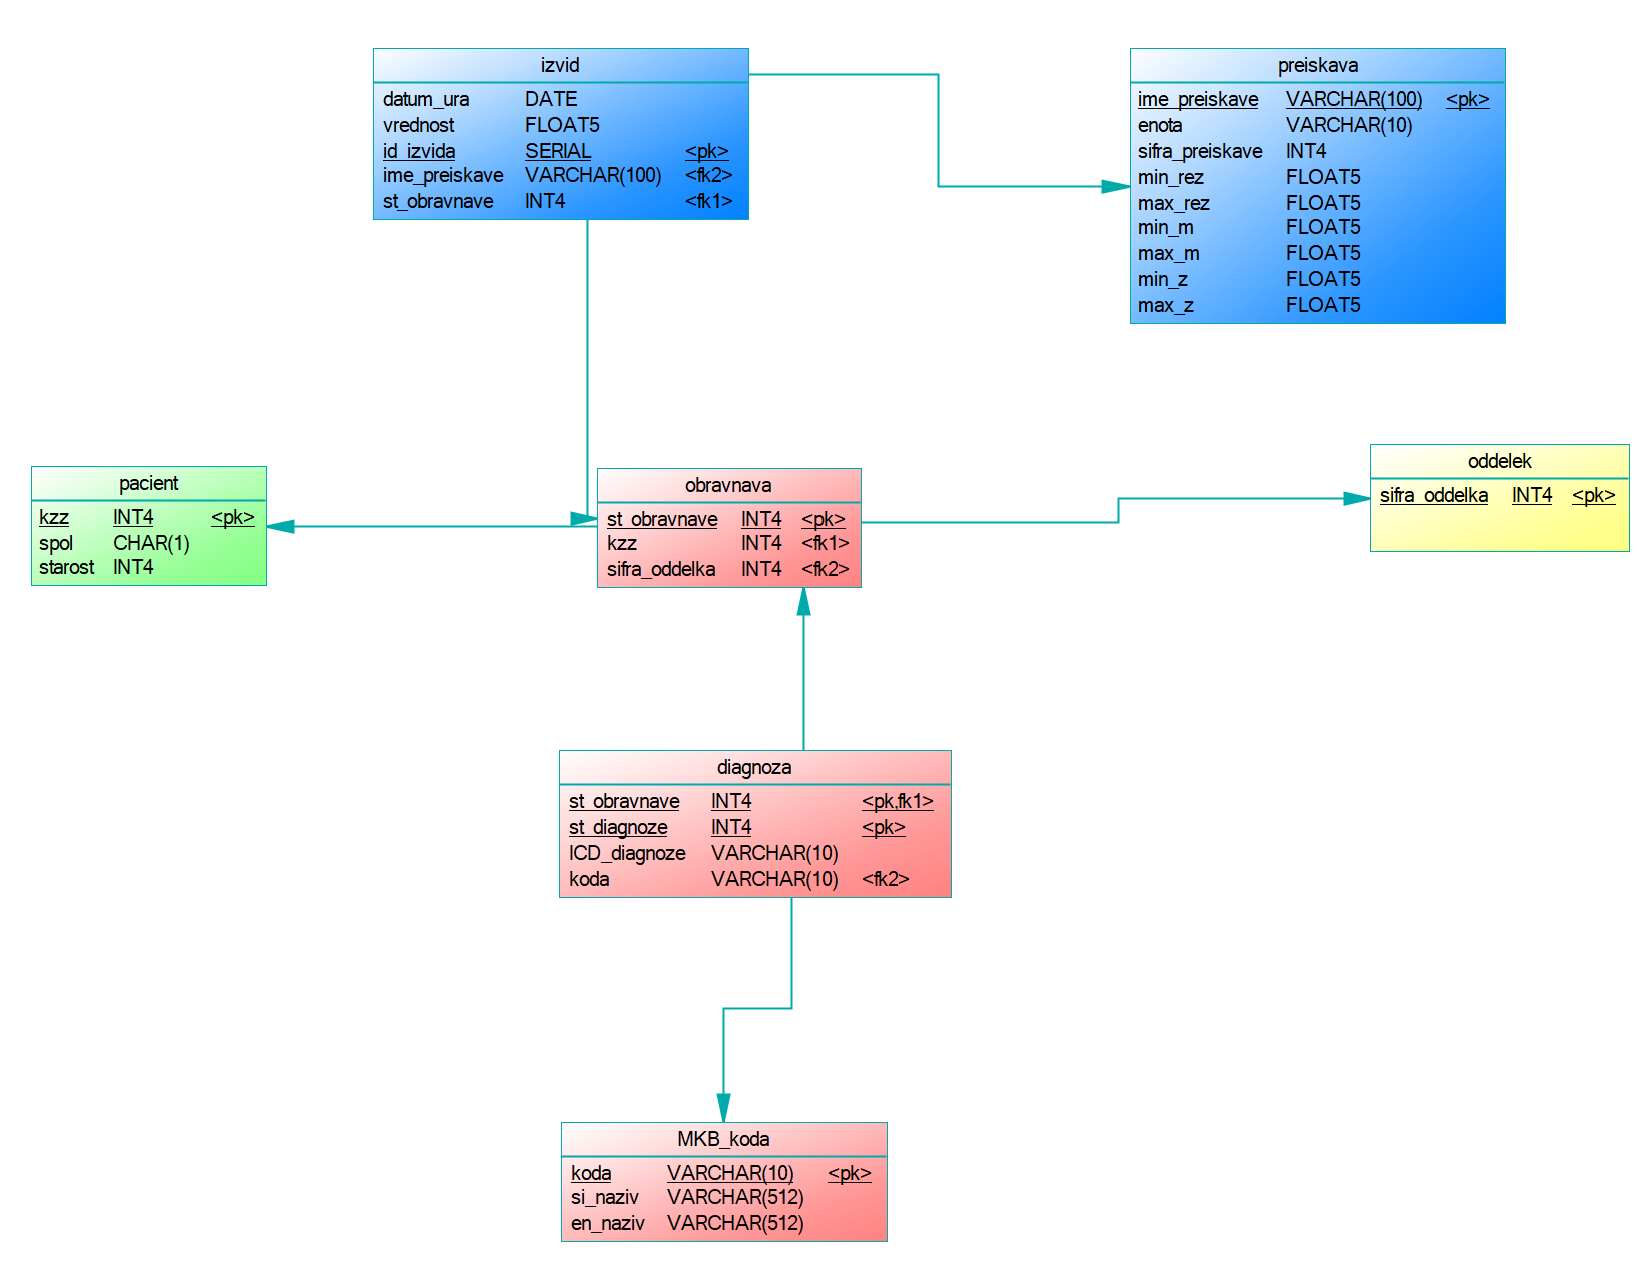
\includegraphics[width=\linewidth]{./pics/fizicni-postgres.png}
   \caption{Fizični model podatkovne baze za PostgreSQL}
\end{figure}
Skripta za ustvarjanje podatkovne baze je shranjena v datoteki \textit{\underline{./sql-skripte/postgres-init.sql}}.

\pagebreak
\subsection{Microsoft SQL Server}
\begin{figure}[htb]
   \noindent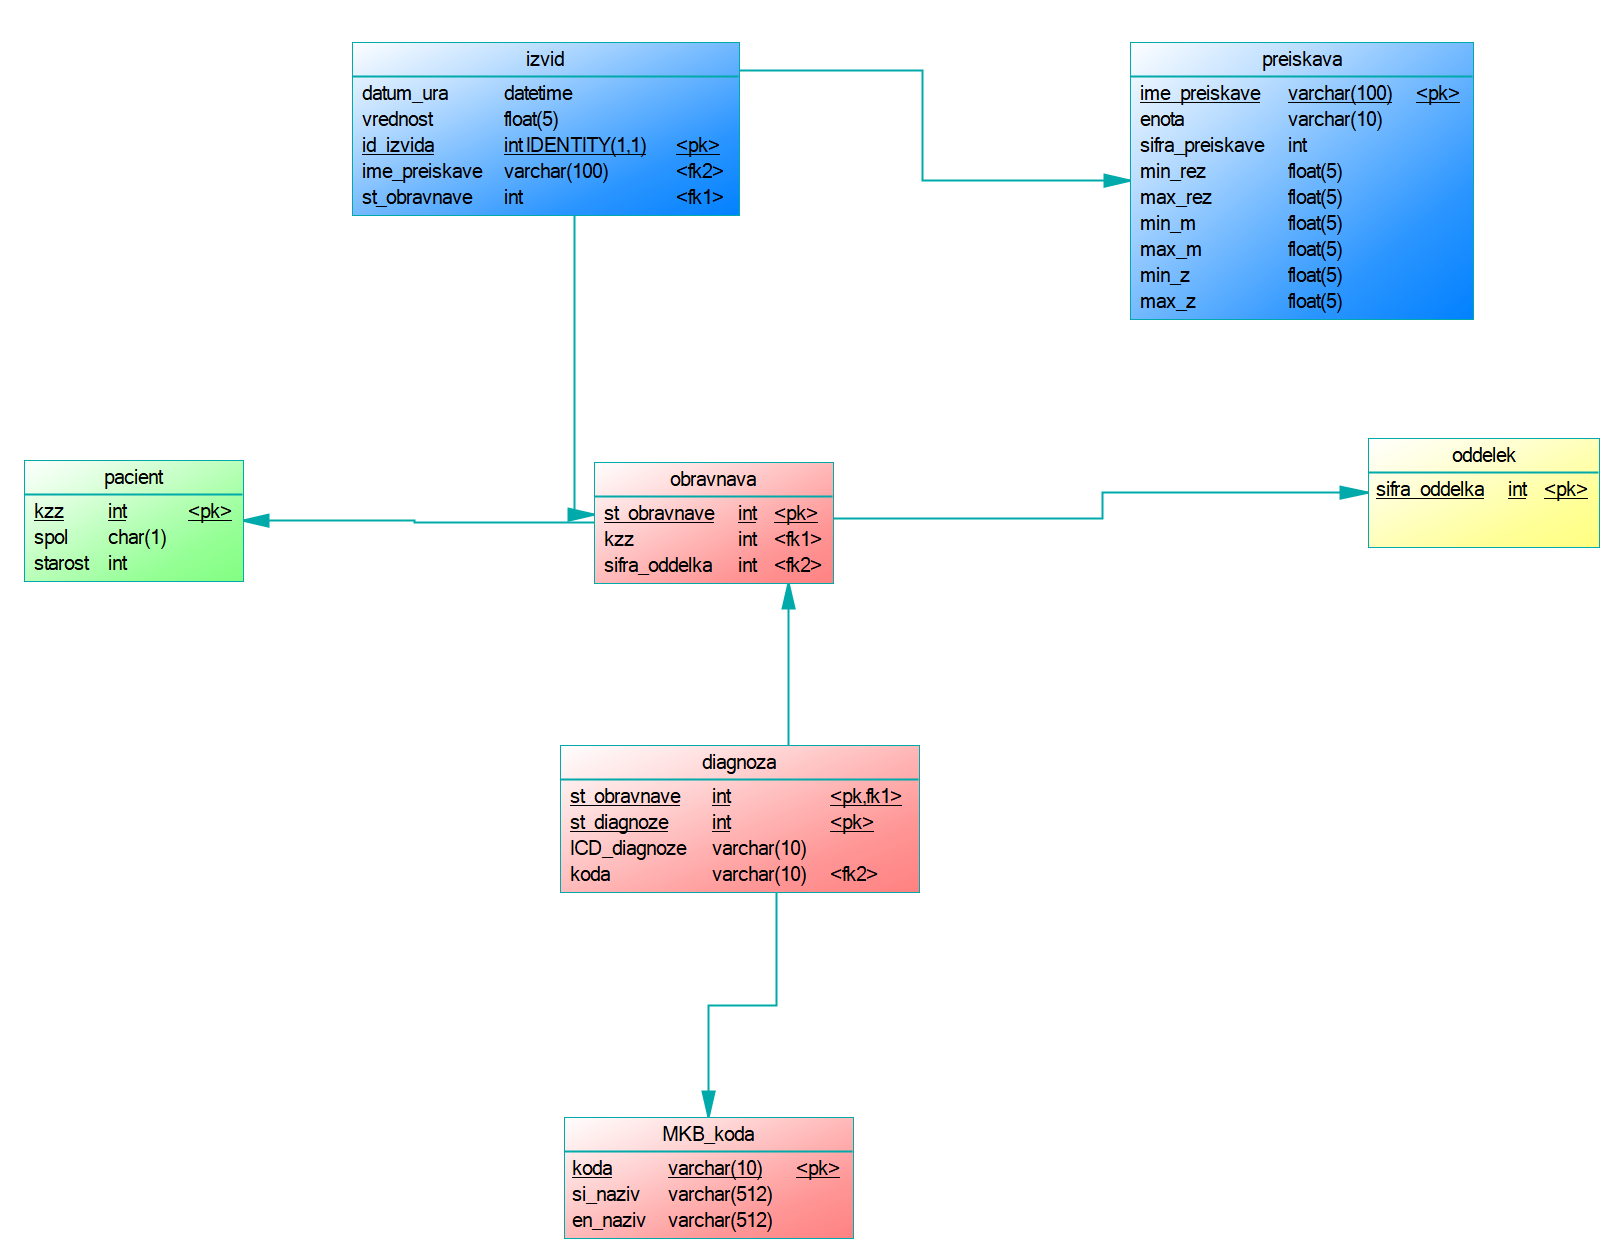
\includegraphics[width=\linewidth]{./pics/fizicni-mssql.png}
   \caption{Fizični model podatkovne baze za MS SQL Server}
\end{figure}
Skripta za ustvarjanje podatkovne baze je shranjena v datoteki \textit{\underline{./sql-skripte/mssql-init.sql}}.

\chapter{Testiranje}

\section{Vstavljanje (velike količine) zapisov v podatkovno bazo}

V podatkovno bazo se je vstavilo skupaj 1 028 883 zapisov. Vstavljanje je potekalo prek Python skripte filanje.py po postopku: 

\begin{enumerate}
   \item Iz csv (coma seperated values) datoteke je program prebral vrstico, jo razdelil in pretvoril v pravilen zapis spremenljivke (s pomočjo vgrajenih ali pomožnih funkcij)
   \item Program shrani trenutni sistemski čas
   \item Program izvede INSERT
   \item Program od trenutnega sistemskega časa odšteje sistemski čas iz točke 3 in ga prišeje k števcu skupnega časa 
   \item Program se premakne na naslednjo vrstico csv datoteke
   \item Ko program obdela vse datoteke, funkcija vrne celoten seštevek časov izvajanja
\end{enumerate}
Test se je avomatsko izvedel desetkrat na vseh testnih bazah.
Po polnjenju vseh treh podatkovnih baz je program podatkovne baze izpraznil pri čemer je bil uporabljen ukaz \textit{DELETE * FROM |ime tabele| }. 
\\\\
Pri obdelavi rezultatov se najboljši in najslabši čas nista upoštevala, iz ostalih pa se je izračunalo povprečje.

\begin{center}
   \begin{tabular}{||c|c|c|c||}
      \hline
      \textbf{SUPB} & \textbf{Najboljši čas [s]} & \textbf{Najslabši čas [s]} & \textbf{Standardni odklon} \\
      \hline
      \hline
      MariaDB & 482,683 & 563,107 & 5,792 \\
      PostgreSQL & 512,716 & 520,791 & 2,170 \\
      Microsoft SQL Server & 592,745 & 608,040 & 4,557 \\
      MySQL & 619,255 & 630,775 & 5,792\\
      \hline
   \end{tabular}
\end{center}

Ob tem gre poudariti, da se je pri vseh uporabljal \textit{običajen INSERT} in ne kakšna posebna oblika vstavljanja velike količine podatkov (npr. \textit{BULK INSERT} pri Microsoft SQL Server).
\\\\
Iz zgoraj navedenih rezultatov se, kot je zapisano v sekciji 1.4.1, določi točke po naslednjem ključu:

\begin{center}
   \begin{tabular}{||c|c|c|c||}
      \hline
      \textbf{SUPB} & Povprečje [ms] & Odstotek točk [\%] & Število točk\\
      \hline
      \hline
      MariaDB & 484 050 & 100 & 25\\
      PostgreSQL & 515 921 & 93,8 & 23,5\\
      Micorsoft SQL Server & 596 453 & 81,2 & 20,3\\
      MySql & 623 806 & 77,6 & 19,4\\
      \hline
   \end{tabular}
\end{center}

\section{Brisanje (velike količine) podatkov iz podatkovne baze}
Brisanje podatkov je potekalo avtomatsko z uporabo Python skripte \textit{filanje.py}. Testiranje se je izvedlo destkrat.
\\\\

Testiranje je potekalo po naslednjem postopku:
\begin{enumerate}
   \item Program izvede ukaz s katerim pridobi imena vseh tabel v podatkovni bazi
      \item Program shrani trenutni sistemski čas
      \item Program izvede ukaz \textit{DELETE FROM |ime-tabele|}
      \item Program od trenutnega sistemskega časa odšteje shranjen čas
   \item Program vrne seštevek vsote časov izvajanja funkcije brisanja podatkov
\end{enumerate}

\pagebreak
Rezultati izračunani iz povprečja so naslednji:
\begin{center}
   \begin{tabular}{||c|c|c|c||}
      \hline
      \textbf{SUPB} & \textbf{Povprečje [ms]} & \textbf{Odstotek točk [\%] } & \textbf{Število točk}\\
      \hline
      \hline
      Microsoft SQL Server & 1087 & 100 & 25\\
      PostgreSQL & 1490 & 72,9 & 18,2\\
      MariaDB & 2418 & 45,0 & 11,2\\
      MySQL & 5373 & 20,2 & 5,1\\
      \hline
   \end{tabular}
\end{center}

Iz zgornjih rezultatov lahko sklepamo, da je brisanje podatkov iz podatkovne baze veliko hitrejši postopek od vstavljanja.
Ravno zaradi tega so relativne razlike med testiranimi SUPB-ji izjemno velike v primerjavi z razlikami pri vstavljanju, čeprav
so absolutne razlike (predvsem med MS SQL Server in PostgreSQL) zanemarljive.

\section{Branje podatov iz podatkovne baze}
\subsection{Povezovanje tabel in primerjava med \textit{WHERE} in \textit{INNER JOIN}}

\paragraph{SQL poizvedba}
Poizvedba za vsakega izmed pacientov prikaže pacientovo številko zdravstvenega zavarovanja, spol, številko obravnave
ter kakšna vrsta preiskave je bila opravljena in njeno vrednost. V testiranju sta bili uporabljeni dve različni poizvedbi
ena z uporabo \textit{INNER JOIN} (poizvedba 1) in druga z uporabo \textit{WHERE} stavka (poizvedba 2).
\begin{lstlisting}[language = SQL]
Poizvedba 1:
   select
      p.kzz,
      p.spol,
      o.st_obravnave,
      i.ime_preiskave,
      i.vrednost
   from pacient p
   inner join obravnava o on o.kzz = p.kzz
   inner join izvid i on i.st_obravnave=o.st_obravnave
   order by p.kzz, o.st_obravnave
\end{lstlisting}
\pagebreak
\begin{lstlisting}[language = SQL]
Poizvedba 2:
   select
       p.kzz,
       p.spol,
       o.st_obravnave,
       i.ime_preiskave,
       i.vrednost
   from
        pacient p,
        obravnava o,
        izvid i
   where
       p.kzz = o.kzz and
       o.st_obravnave = i.st_obravnave
   order by p.kzz, o.st_obravnave
\end{lstlisting}

\paragraph{Rezultati poizvedbe 1 (\textit{INNER JOIN})}
Test se je izvedel desetkrat, avtomatsko z uporabo Python skripte \textit{poizvedbe.py} za vse štiri podatkovne baze.

\begin{center}
   \begin{tabular}{||c|c|c|c||}
      \hline
      \textbf{SUPB} & \textbf{Najboljši [ms]} & \textbf{Najslabši [ms]} & \textbf{Povprečje [ms]}\\
      \hline
      \hline
      Microsoft SQL Server & 312 & 361 & 0,016 \\
      MySql & 701 & 838 & 0,038 \\
      PostgreSQL & 879 & 1040 & 0,058\\
      MariaDB & 1188 & 1374 & 0,057 \\
      \hline
   \end{tabular}
\end{center}
Primerjava hitrsoti izvedbe SQL stavka z uporabo \textit{INNER JOIN}

\paragraph{Rezultati poizvedbe 1 (\textit{WHERE})}
\begin{center}
   \begin{tabular}{||c|c|c|c||}
      \hline
      \textbf{SUPB} & \textbf{Najboljši [ms]} & \textbf{Najslabši [ms]} & \textbf{Standardni odklon}\\
      \hline
      \hline
      Microsoft SQL Server & 303 & 375 & 0,021 \\
      MySql & 702 & 729 & 0,026 \\
      PostgreSQL & 885 & 973 & 0,005\\
      MariaDB & 1204 & 1223 & 0,008 \\
      \hline
   \end{tabular}
\end{center}
Primerjava hitrsoti izvedbe SQL stavka z uporabo \textit{WHERE}

\pagebreak
Razlike med hitrostjo poizvedb pri uporabi \textit{WHERE} in \textit{INNER JOIN} so pri vseh štirih bazah zanemarljive:

\begin{center}
   \begin{tabular}{||c|c|c|c||}
      \hline
      \textbf{SUPB} & \textbf{\textit{INNER JOIN} [ms]} & \textbf{\textit{WHERE} [ms]} & \textbf{Razlika [\%]}\\
      \hline
      \hline
      Microsoft SQL Server & 334 & 336 & 0,5 \\
      MySql & 725 & 710 & -2,1 \\
      PostgreSQL & 925 & 909 & -1,8\\
      MariaDB & 1237 & 1212 & -2,1 \\
      \hline
   \end{tabular}
\end{center}
Prikaz razlike v povprečni hitrosti izvedbe SQL poizvedbe z uporabo \textit{INNER JOIN} in \textit{WHERE} stavka.

\paragraph{Določitev točk} Čeprav se poizvedba deli na dve sintaktično različni, je razultat obeh poizvedb identičen. Kot takega
ga torej štejemo kot eno postavko izračuna točk, pri čemer se upošteva boljši rezultat obeh poizvedb.

\begin{center}
   \begin{tabular}{||c|c|c|c||}
      \hline
      \textbf{SUPB} & \textbf{Povprečje [ms]} & \textbf{Odstotek točk [\%]} & \textbf{Število točk}\\
      \hline
      \hline
      Microsoft SQL Server & 334 & 100 & 50 \\
      MySql & 710 & 47,0 & 23,5 \\
      PostgreSQL & 909 & 36,7 & 18,4\\
      MariaDB & 1212 & 27,6 & 13,8 \\
      \hline
   \end{tabular}
\end{center}

\subsection{Uporaba funkcije \textit{COUNT} v povezanih tabelah in predpomnjenje}
Test se je izvedel desetkrat, avtomatsko z uporabo Python skripte \textit{poizvedbe.py} za vse štiri podatkovne baze.

\paragraph{SQL poizvedba}
Poizvedba izpiše ime preiskave in število izvidov, katerih vrednost je višja od priporočene vrednosti glede na spol.
Izpis je urejen padajoče po številu prekoračenih izvidov.
\pagebreak
\begin{lstlisting}[language = SQL]
select
   i.ime_preiskave,
   count(i.ime_preiskave)
from
   izvid i
inner join obravnava o on 
      i.st_obravnave = o.st_obravnave
inner join pacient p 
      on p.kzz = o.kzz
inner join preiskava p2 
      on i.ime_preiskave = p2.ime_preiskave
where
   (p.spol = 'M' and p2.max_m <= i.vrednost 
      and p2.max_m is not null) 
   or
   (p.spol = 'Z' and p2.max_z <= i.vrednost 
      and p2.max_z is not null)
group by i.ime_preiskave
order by count(i.ime_preiskave) desc
\end{lstlisting}

\begin{center}
   \begin{tabular}{||c|c|c|c||}
      \hline
      \textbf{SUPB} & \textbf{Najboljši [ms]} & \textbf{Najslabši [ms]} & \textbf{Standardni odklon}\\
      \hline
      \hline
      MariaDB & 1 & 1166 & 0,350 \\
      PostgreSQL & 314 & 416 & 0,034 \\
      Microsoft SQL Server & 490 & 584 & 0,028 \\
      MySql & 1534 & 2567 & 0,379\\
      \hline
   \end{tabular}
\end{center}

\begin{center}
   \begin{tabular}{||c|c|c|c||}
      \hline
      \textbf{SUPB} & \textbf{Povprečje [ms]} & \textbf{Odstotek točk [\%]} & \textbf{Število točk}\\
      \hline
      \hline
      MariaDB & 118 & 100 & 50 \\
      PostgreSQL & 362 & 32,4 & 16,2\\
      Microsoft SQL Server & 518 & 22,7 & 11,2 \\
      MySql & 1704 & 6,5 & 3,4 \\
      \hline
   \end{tabular}
\end{center}

V tem testu se je prvič videla moč predpomnjenja, ki ga uporablja MariaDB, ki si shranjuje rezultate poizvedbe.
Baza naslednjič servira že predpomnjene podatke in ne izvaja SQL poizvedbe ponovno. To je uporabno predvsem v podatkovnih bazah, kjer
je pogostejše branje iz baze, kot je pisanje v njo.

\pagebreak
\subsection{Uporaba funkcij \textit{COUNT, MAX, MIN, AVG}}
Test se je izvedel desetkrat, avtomatsko z uporabo Python skripte \textit{poizvedbe.py} za vse štiri podatkovne baze.

\paragraph{SQL poizvedba}
Poizvedba izpiše število opravljenih preiskav, z minimalno, maksimalno in povprečno vrednostjo, kjer
je število izvedb večje od 200 in je povprečna vrednost večja od polovice maksimalne vrednosti.
\begin{lstlisting}[language = SQL]
Select 
   ime_preiskave, 
   count(vrednost), 
   min(vrednost), 
   max(vrednost), 
   avg(vrednost)
from izvid
group by ime_preiskave
having 
   count(vrednost) > 200 and 
   avg(vrednost) * 2 <= max(vrednost)
order by count(vrednost) desc, ime_preiskave asc
\end{lstlisting}

\begin{center}
   \begin{tabular}{||c|c|c|c||}
      \hline
      \textbf{SUPB} & \textbf{Najboljši [ms]} & \textbf{Najslabši [ms]} & \textbf{Standardni odklon}\\
      \hline
      \hline
      MariaDB & 1 & 622 & 0,186 \\
      PostgreSQL & 237 & 307 & 0,020 \\
      Microsoft SQL Server & 230 & 316 & 0,028 \\
      MySql & 898 & 984 & 0,029\\
      \hline
   \end{tabular}
\end{center}

\begin{center}
   \begin{tabular}{||c|c|c|c||}
      \hline
      \textbf{SUPB} & \textbf{Povprečje [ms]} & \textbf{Odstotek točk [\%]} & \textbf{Število točk}\\
      \hline
      \hline
      MariaDB & 63 & 100 & 50 \\
      Microsoft SQL Server & 265 & 23,7 & 11,9 \\
      PostgreSQL & 362 & 17,4 & 8,7\\
      MySql & 927 & 6,7 & 3,4 \\
      \hline
   \end{tabular}
\end{center}

Zopet ima veliko prednost MariaDB, predvsem zaradi predpomnjenja, v kolikor le tega ne bi uporabljali (ali bi se med branji zgodilo novo pisanje) bi čas poizvedbe bil primerjiv najslabšemu rezultatu v testiranju,

\pagebreak
\subsection{Korelirane gnezdene SQL poizvedbe}
Test se je izvedel desetkrat, avtomatsko z uporabo Python skripte \textit{poizvedbe.py} za vse štiri podatkovne baze.

\paragraph{SQL poizvedba}
Poizvedba poišče vse diagnoze v katerih se nahaja ključna beseda, v gnezdenih skriptah pridobimo
najmaljšo, najstarejšo in povprečno starost pacientov z iskano diagnozo.

\begin{lstlisting}[language = SQL]
   select m.si_naziv, count(o.st_obravnave) as Stevilo,
   (
       select min(p1.starost)
           from
               pacient p1,
               obravnava o1,
               diagnoza d1,
               MKB_koda m1
           Where
               p1.kzz = o1.kzz and
               d1.st_obravnave = o1.st_obravnave and
               d1.icd_diagnoze = m1.koda and
               m1.si_naziv = m.si_naziv
   ) as min,
   (
       select max(p1.starost)
           from
               pacient p1,
               obravnava o1,
               diagnoza d1,
               MKB_koda m1
           Where
               p1.kzz = o1.kzz and
               d1.st_obravnave = o1.st_obravnave and
               d1.icd_diagnoze = m1.koda and
               m1.si_naziv = m.si_naziv
   ) as max,
   (
       Select avg(p1.starost)
           from
               pacient p1,
               obravnava o1,
               diagnoza d1,
               MKB_koda m1
           Where
               p1.kzz = o1.kzz and
               d1.st_obravnave = o1.st_obravnave and
               d1.icd_diagnoze = m1.koda and
               m1.si_naziv = m.si_naziv
   ) as povprecje
from pacient p
   inner join obravnava o 
      on p.kzz = o.kzz
   Inner join diagnoza d 
      on o.st_obravnave = d.st_obravnave
   inner join MKB_koda m 
      on m.koda = d.icd_diagnoze
   inner join izvid i 
      on d.st_obravnave = i.st_obravnave
   inner join preiskava p2 
      on i.ime_preiskave = p2.ime_preiskave
   where
       p.starost between 21 and 40 and
       m.si_naziv like '%tr_en%'
   group by m.si_naziv, p.starost
   order by count(o.st_obravnave) desc
\end{lstlisting}

\begin{center}
   \begin{tabular}{||c|c|c|c||}
      \hline
      \textbf{SUPB} & \textbf{Najboljši [ms]} & \textbf{Najslabši [ms]} & \textbf{Standardni odklon}\\
      \hline
      \hline
      Microsoft SQL Server & 374 & 568 & 0,058 \\
      PostgreSQL & 7045 & 7243 & 0,064 \\
      MariaDB & 1 & 164 669 & 49,400 \\
      MySql & 139 951 & 144 340 & 1,209 \\
      \hline
   \end{tabular}
\end{center}

\begin{center}
   \begin{tabular}{||c|c|c|c||}
      \hline
      \textbf{SUPB} & \textbf{Povprečje [ms]} & \textbf{Odstotek točk [\%]} & \textbf{Število točk}\\
      \hline
      \hline
      Microsoft SQL Server & 407 & 100 & 50 \\
      PostgreSQL & 7100 & 5,8 & 2,9\\
      MariaDB & 16 486 & 2,4 & 1,2 \\
      MySql & 1704 & ~0,1 & 0,1 \\
      \hline
   \end{tabular}
\end{center}

Test preverja predvsem hitrost izvedbe gnezdenih SQL poizvedb in primerjave nizov znakov. 
Izkaže se, da Microsoft SQL server uporablja veliko bolj optimizirano proceduro za izvajanje takšne poizvedbe. Hkratu
se zopet izkaže kakšno moč ima predpomnjenje, ki ga uporablja MariaDB, vendar je ob tem potrebno predpostaviti, da se
med samimi bralnimi poizvedbami ne izvede pisanje (nov zapis ali posodabljanje), zaradi česar bi predpomnjen rezultat postal neveljaven.

\section{Posodabljanje zapisov v podatkovni bazi}

\paragraph{SQL poizvedba}
Poizvedba za vsako preiskavo, kjer je referenčna vrednost ženskega spola \textit{NULL} posodobi le-to vrednost, na referenčno vrednost za moške.

\begin{lstlisting}[language = SQL]
update preiskava
   set min_z = min_m, max_z = max_m
where min_z is null and max_z is null
\end{lstlisting}

\begin{center}
   \begin{tabular}{||c|c|c|c||}
      \hline
      \textbf{SUPB} & \textbf{Vstavljanje [ms]} & \textbf{Commit [ms]} & \textbf{Skupaj [ms]}\\
      \hline
      \hline
      MySql & 3 & 2 & 5\\
      Microsoft SQL Server & 7 & 3 & 10 \\
      PostgreSQL & 11 & 10 & 21 \\
      MariaDB & 15 & 9 & 24 \\
      \hline
   \end{tabular}
\end{center}

\begin{center}
   \begin{tabular}{||c|c|c|c||}
      \hline
      \textbf{SUPB} & \textbf{Povprečje [ms]} & \textbf{Odstotek točk [\%]} & \textbf{Število točk}\\
      \hline
      \hline
      MySql & 5 & 100 & 50 \\
      Microsoft SQL Server & 10 & 50 & 25 \\
      PostgreSQL & 21 & 23,8 & 11,9\\
      MariaDB & 24 & 20,8 & 10,4 \\
      \hline
   \end{tabular}
\end{center}

Enostavno posodabljanje se izkaže za hitro operacijo. Še enkrat znova vidimo, da so vse podatkovne baze približno enako (dobro) optimizirane za izvajanje enostavnih poizvedb/operacij. Razlike se pojavljajo šele pri večji količini podatkov in/ali bolj kompliciranih poizvedbah.


\chapter{Zaključek}

\section{Seštevek točk performančnih testov}

\begin{center}
   \begin{tabular}{||c|c|c|c|c||}
      \hline
      \textbf{Test} & \textbf{MSSQL Server} & \textbf{MariaDB} & \textbf{PostgreSQL} & \textbf{MySQL}\\
      \hline
      \hline
      Vstavljanje & 20,3 & 25 & 23,5 & 19,4\\
      Brisanje & 25 & 11,5 & 18,2 & 5,1\\
      Branje 1 & 50 & 18,4 & 13,8 & 23,5\\
      Branje 2 & 11,2 & 50 & 16,2 & 3,4\\
      Branje 3 & 11,9 & 50 & 8,7 & 3,4\\
      Branje 4 & 50 & 1,2 & 2,9 & 0,1\\
      Posodabljanje & 25 & 10,4 & 11,9 & 50\\
      \hline
      \hline
      \textbf{Vsota} & 193,4 & 166,5 & 94,9 & 104,9\\
      \hline
   \end{tabular}
\end{center}

\paragraph{Razumevanje rezultatov performančnih testov}
Izvedeni testi v okviru seminarkse naloge zagotavljajo primerjivo testno okolje za vse podatkovne baze,
vendar ne zagotavljajo optimalne konfiguracije baz. Ravno tako v testih niso uporabljene posebne inačice SQL jezika,
ampak se (kjer je to mogoče) uporablja splošno sprejeta oblika SQL jezika \textit{(ne uporablja se posebnih ukazov kot so INSERT IGNORE ali BULK INSERT)},
ravno tako so rezultati močno podvrženi sistematičnosti testov, ki omogočajo višjo performanso podatkovnih baz z vgrajenim predpomnjenjem (izrazito MariaDB).

\pagebreak

\section{Poraba sistemskih virov}
Čeprav so bili testi izvedeni ob predpostavki, da ima SUPB dovolj zmogljivo strojno arhitekturo ter poraba sistemski virov ni vplivala na točkovanje, se je ob testiranju izvajal tudi monitoring porabe sistemskih virov.

\subsection{Poraba CPU}
V času, ko je izbrani SUPB izvajal transakcije, je bila CPU poraba izbrane docker slike višja, približno 50\% pri vseh testiranih.

V času, ko izbran SUPB ni izvajal operacij, je bila CPU poraba izbrane docker slike zanemarljiva (do 5\%).

\subsection{Poraba delovnega pomnilnika}
Večje razlike se pojavijo pri uporabi delovnega pomnilnika, saj imajo različni SUPB-ji arzlične strategije uporabe.

Najmanj delovnega pomnilnika (tako v času izvajanja operacij kot v času neizvajanja) porablja PostgreSQL, približno 10MB.
Sledita mu MariaDB (350MB "mirovanje", 500MB v času izvajanja daljših operacij) in MySQL (500MB "mirovanje", 700MB v času izvajanja daljših operacij), daleč največ pomnilnika pa porabi Microsoft SQL Server s porabo približno 1,3GB v "mirovanju"  in 1,8GB v izvajanju večjih in daljših operacij (npr. vstavljanje).

Vse porabe se bistveno ne spreminjajo od prve izvedene operacije po zagonu. Torej izbrani SUPB po zasedbi pomnilnika, le tega ne sprosti več (razlika je vidna samo pri MSSQL, kjer je poraba tako ali drugače izjemno velika).

\pagebreak
\section{Izbira SQL podatkovne baze}
Dasiravno je in tudi bo izbira podatkovne baze odvisna od želja in izkušenj programerjev, naročnikov in uporabnikov informacijske rešitve,
lahko iz performančnih testov potegnemo nekaj zaključkov.

\subsection{Microsoft SQL Server}
Microsoft SQL Server ima izmed 4 testiranih najboljšo performanco, saj je poleg hitrega vstavljanja in brisanja,
povprečno hiter tudi pri pososdabljanju podatkov v tabelah. Najboljšo optimiziranost pa zagotavlja tudi pri branju podatkov
z uporabo gnezdenih SQL poizvedb in poizvedb z uporabo agregatnih funkcij, brez prevelikega zanašanja na predpomnjenje.

Največja težava MSSQL Serverja je njegov SQL jezik, ki se predvsem pri kreiranju in brisanju tabel močno razlikuje od ostalih testiranih.
V velikem produkcijskem okolju moramo tudi predvideti možnost, da brezplačna verzija ne bo omogočala dovolj funkcij, ki so potrebne pri takšni vrsti sistemov.

\subsection{MySQL}
Čeprav je MySQL "de-facto"\ standard v industriji se je (presenetljivo) izkazal za najmanj optimiziranega.
Edina kategorija v kateri je izstopal je bila posodabljanje podatkov. 

Pri naslednjem projektu, je zato mogoče bolje razmisliti o smiselni alternativi.

\subsection{MariaDB}
MariaDB je pogostokrat označena kot mlajša sestra MySQL (kar tudi je), vendar se je v testih izkazala kot boljša alternativa, saj je konstantno dosegala performančno boljše rezultate.
\\\\
Zaradi svojega velikega zanašanja na predpomnilnik je najboljša izbira za baze, kjer se zapisi dogajajo dokaj redko, veliko pa je ponovljivih branj.
Zaradi podobnosti zgradbe z MySQL je prehod med eno in drugo instanten, saj uporabljata (večino) enake gonilnike kakor
tudi SQL jezik.

\pagebreak

\subsection{PostgreSQL}
PostgreSQL se izkaže za nekoliko slabšo alternativo vsem zgoraj omenjenim podatkovnim bazam, vendar vseeno zagotavlja povprečno performanco.
\\\\
PostgreSQL je vseeno odlična izbira za sisteme, ki so omejeni s sistemskimi viri, predvsem z delovnim pomnilnikom, saj uporablja najbolj rigorozno strategijo in zasede (tako ob izvajanju operacij kot mirovanju) daleč najmanj delovnega pomnilnika.

\section{Zaključek}
Izbira SUPB-ja bo še naprej ostala primarno odvisna od kompetenc naročnika-izvajalca, vendar se vseeno zdi, da ima vsaka podatkovna baza svoje prednosti in slabosti, ki niso nujno povezane (samo) z golo performanco.
\\\\
Programerji pa si lahko kot izziv vedno znova pri svojih projektih izbirajo drugo rešitev, ki jim omogoča, da spoznajo alternative kakor tudi možnosti, ki jih alternative ponujajo.


\begin{tabular}{|c|c|c|c|} \hline $Y\ \backslash\ X$& $0$ & $1$ & $2$ \\ \hline $-1$& $0$ & $1/4$& $0$ \\ \hline $0$& $0$ & $1/4$ & $1/4$ \\ \hline $1$& $1/4$& $0$ & $0$ \\ \hline \end{tabular}

\end{document}